\documentclass[main.tex]{subfiles}
\begin{document}

\chapter{Unbiasedness, Consistency and the MSE Decomposition}\label{ch:nokta-tahmin}\chaptermark{Unbiasedness, Consistency and MSE}

With this chapter we move from probability theory to statistical inference. The distribution is now unknown; we assume that it belongs to a parametric family $\{f(\cdot;\theta):\theta\in\Theta\}$ and make inferences about $\theta$ (or a function $g(\theta)$ of it) from the observed sample $\X=(X_1,\dots,X_n)$. The first question is: what is a ``good'' estimator\index{estimator@estimator}? In this chapter we discuss bias, variance and mean squared error\index{mean squared error mse@mean squared error (MSE)} (MSE); we see that unbiasedness, while a virtue, is not the only criterion; and we introduce consistency\index{consistency@consistency}, which measures large-sample behaviour. Finally, we prove Stein's paradox\index{stein s paradox@Stein's paradox}, which shows that in multidimensional problems even the most natural estimator can be inadmissible\index{admissibility@admissibility}.

\section{Definitions}

\begin{definition}[Statistic and Estimator]\index{estimator@estimator|textbf}
A measurable function $T=T(\X)$ of the sample that does not depend on the unknown parameter is called a \emph{statistic}. A statistic used to estimate $g(\theta)$ is called an \emph{estimator} of $g(\theta)$, and its observed value $T(\x)$ an \emph{estimate}.
\end{definition}

\begin{definition}[Bias and MSE]\index{mean squared error mse@mean squared error (MSE)|textbf}
Let $\hat\theta$ be an estimator of $\theta$:
\[
\Bias_\theta(\hat{\theta}) = \E_\theta[\hat{\theta}] - \theta,\qquad \MSE_\theta(\hat{\theta}) = \E_\theta[(\hat{\theta} - \theta)^2].
\]
If $\Bias_\theta(\hat\theta)=0$ for every $\theta\in\Theta$, $\hat\theta$ is \emph{unbiased}. If $\lim_{n\to\infty}\Bias_\theta(\hat\theta_n)=0$, it is \emph{asymptotically unbiased}.
\end{definition}

\begin{definition}[Consistency]\index{consistency@consistency|textbf}
A sequence of estimators $\{\hat\theta_n\}$ is \emph{(weakly) consistent} if $\hat\theta_n\pto\theta$ (under $\P_\theta$) for every $\theta\in\Theta$. It is \emph{strongly consistent} if $\hat\theta_n\asto\theta$, and \emph{MSE-consistent} if $\MSE_\theta(\hat\theta_n)\to0$.
\end{definition}

\begin{definition}[Loss, Risk and Admissibility]\label{def:risk}\index{admissibility@admissibility|textbf}
A \emph{loss function\index{loss function@loss function}} $L:\Theta\times\R\to[0,\infty)$ measures the cost of the estimate $a$ when the true value is $\theta$. The \emph{risk function\index{risk function@risk function}} of $\hat\theta$ is $R(\theta,\hat\theta)=\E_\theta[L(\theta,\hat\theta(\X))]$. Under squared loss $L(\theta,a)=(a-\theta)^2$ the risk is the MSE.
If $R(\theta,\hat\theta_1)\le R(\theta,\hat\theta_2)$ for every $\theta$, with strict inequality for at least one $\theta$, then $\hat\theta_1$ \emph{dominates} $\hat\theta_2$. An estimator dominated by no other estimator is called \emph{admissible}.
\end{definition}

\begin{definition}[Method of Moments]\label{def:momentler}
Let $\theta=(\theta_1,\dots,\theta_k)$ and $\mu_j'(\theta)=\E_\theta[X^j]$. The \emph{method of moments\index{method of moments@method of moments}} (MM) estimator is the solution in $\theta$ of the system
\[
\mu_j'(\theta)=m_j'=\frac1n\sum_{i=1}^n X_i^j,\qquad j=1,\dots,k .
\]
\end{definition}

\section{Main Theorems and Proofs}

\begin{theorem}[Bias--Variance Decomposition of the MSE]\label{thm:mse-ayrisim}\index{mean squared error mse@mean squared error (MSE)}
If $\E_\theta[\hat\theta^2]<\infty$, then
\[
\MSE_\theta(\hat{\theta}) = \Var_\theta(\hat{\theta}) + [\Bias_\theta(\hat{\theta})]^2.
\]
\end{theorem}
\begin{proof}
Write $\hat{\theta} - \theta = (\hat{\theta} - \E_\theta[\hat{\theta}]) + (\E_\theta[\hat{\theta}] - \theta)$. The second term is a constant. Squaring and taking expectations,
\[
\MSE_\theta(\hat\theta)=\E_\theta(\hat\theta-\E_\theta\hat\theta)^2+2(\E_\theta\hat\theta-\theta)\underbrace{\E_\theta[\hat\theta-\E_\theta\hat\theta]}_{=0}+(\E_\theta\hat\theta-\theta)^2,
\]
i.e.\ the cross term vanishes: $2\E[(\hat{\theta}-\E[\hat{\theta}])(\E[\hat{\theta}]-\theta)] = 0$.
\end{proof}

\begin{remark}
This decomposition is the formula behind the \emph{bias--variance\index{bias variance decomposition@bias--variance decomposition} trade-off} of statistics and machine learning: if accepting some bias reduces the variance by more, the MSE goes down. Shrinkage\index{shrinkage@shrinkage}, regularisation (ridge\index{ridge regression@ridge regression}, lasso) and Bayes estimators\index{bayes estimator@Bayes estimator}\index{estimator@estimator} rest on this principle.
\end{remark}

Figure~\ref{fig:yan-varyans} shows the two components of the decomposition on a target.

\begin{figure}[ht]
\centering
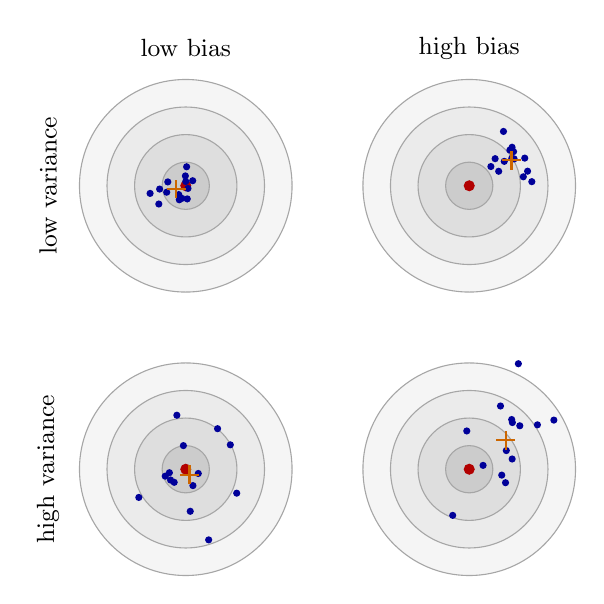
\begin{tikzpicture}[lab/.style={font=\small}]
  \foreach \r/\c in {1.35/gray!8,1.0/gray!16,0.65/gray!26,0.3/gray!40} \fill[\c] (0,0) circle (\r);
  \foreach \r in {1.35,1.0,0.65,0.3} \draw[gray!70] (0,0) circle (\r);
  \fill[red!70!black] (0,0) circle (2pt);
  \fill[blue!60!black] (0.000,0.054) circle (1.3pt);
  \fill[blue!60!black] (-0.049,-0.160) circle (1.3pt);
  \fill[blue!60!black] (-0.082,-0.178) circle (1.3pt);
  \fill[blue!60!black] (0.011,0.241) circle (1.3pt);
  \fill[blue!60!black] (-0.089,-0.112) circle (1.3pt);
  \fill[blue!60!black] (0.088,0.064) circle (1.3pt);
  \fill[blue!60!black] (0.019,-0.167) circle (1.3pt);
  \fill[blue!60!black] (-0.005,0.125) circle (1.3pt);
  \fill[blue!60!black] (-0.242,-0.082) circle (1.3pt);
  \fill[blue!60!black] (-0.342,-0.232) circle (1.3pt);
  \fill[blue!60!black] (-0.332,-0.042) circle (1.3pt);
  \fill[blue!60!black] (-0.228,0.049) circle (1.3pt);
  \fill[blue!60!black] (0.028,-0.034) circle (1.3pt);
  \fill[blue!60!black] (-0.453,-0.097) circle (1.3pt);
  \draw[orange!80!black,thick] (-0.240,-0.041) -- (0.000,-0.041) (-0.120,-0.161) -- (-0.120,0.079);
  \foreach \r/\c in {1.35/gray!8,1.0/gray!16,0.65/gray!26,0.3/gray!40} \fill[\c] (3.6,0) circle (\r);
  \foreach \r in {1.35,1.0,0.65,0.3} \draw[gray!70] (3.6,0) circle (\r);
  \fill[red!70!black] (3.6,0) circle (2pt);
  \fill[blue!60!black] (4.141,0.350) circle (1.3pt);
  \fill[blue!60!black] (3.875,0.244) circle (1.3pt);
  \fill[blue!60!black] (3.974,0.184) circle (1.3pt);
  \fill[blue!60!black] (4.341,0.185) circle (1.3pt);
  \fill[blue!60!black] (4.144,0.489) circle (1.3pt);
  \fill[blue!60!black] (4.045,0.310) circle (1.3pt);
  \fill[blue!60!black] (4.170,0.341) circle (1.3pt);
  \fill[blue!60!black] (3.929,0.344) circle (1.3pt);
  \fill[blue!60!black] (4.395,0.052) circle (1.3pt);
  \fill[blue!60!black] (4.305,0.351) circle (1.3pt);
  \fill[blue!60!black] (4.035,0.690) circle (1.3pt);
  \fill[blue!60!black] (4.287,0.114) circle (1.3pt);
  \fill[blue!60!black] (4.163,0.434) circle (1.3pt);
  \fill[blue!60!black] (4.116,0.453) circle (1.3pt);
  \draw[orange!80!black,thick] (4.017,0.324) -- (4.257,0.324) (4.137,0.204) -- (4.137,0.444);
  \foreach \r/\c in {1.35/gray!8,1.0/gray!16,0.65/gray!26,0.3/gray!40} \fill[\c] (0,-3.6) circle (\r);
  \foreach \r in {1.35,1.0,0.65,0.3} \draw[gray!70] (0,-3.6) circle (\r);
  \fill[red!70!black] (0,-3.6) circle (2pt);
  \fill[blue!60!black] (-0.030,-3.300) circle (1.3pt);
  \fill[blue!60!black] (0.647,-3.904) circle (1.3pt);
  \fill[blue!60!black] (0.091,-3.808) circle (1.3pt);
  \fill[blue!60!black] (0.057,-4.134) circle (1.3pt);
  \fill[blue!60!black] (-0.261,-3.688) circle (1.3pt);
  \fill[blue!60!black] (0.404,-3.085) circle (1.3pt);
  \fill[blue!60!black] (-0.596,-3.958) circle (1.3pt);
  \fill[blue!60!black] (0.291,-4.497) circle (1.3pt);
  \fill[blue!60!black] (-0.208,-3.644) circle (1.3pt);
  \fill[blue!60!black] (0.566,-3.290) circle (1.3pt);
  \fill[blue!60!black] (-0.147,-3.766) circle (1.3pt);
  \fill[blue!60!black] (-0.113,-2.914) circle (1.3pt);
  \fill[blue!60!black] (-0.193,-3.737) circle (1.3pt);
  \fill[blue!60!black] (0.159,-3.654) circle (1.3pt);
  \draw[orange!80!black,thick] (-0.072,-3.670) -- (0.168,-3.670) (0.048,-3.790) -- (0.048,-3.550);
  \foreach \r/\c in {1.35/gray!8,1.0/gray!16,0.65/gray!26,0.3/gray!40} \fill[\c] (3.6,-3.6) circle (\r);
  \foreach \r in {1.35,1.0,0.65,0.3} \draw[gray!70] (3.6,-3.6) circle (\r);
  \fill[red!70!black] (3.6,-3.6) circle (2pt);
  \fill[blue!60!black] (4.061,-3.771) circle (1.3pt);
  \fill[blue!60!black] (4.145,-3.470) circle (1.3pt);
  \fill[blue!60!black] (4.675,-2.976) circle (1.3pt);
  \fill[blue!60!black] (4.139,-2.969) circle (1.3pt);
  \fill[blue!60!black] (3.997,-2.797) circle (1.3pt);
  \fill[blue!60!black] (4.148,-3.007) circle (1.3pt);
  \fill[blue!60!black] (3.569,-3.114) circle (1.3pt);
  \fill[blue!60!black] (3.390,-4.186) circle (1.3pt);
  \fill[blue!60!black] (4.013,-3.675) circle (1.3pt);
  \fill[blue!60!black] (4.224,-2.260) circle (1.3pt);
  \fill[blue!60!black] (3.776,-3.551) circle (1.3pt);
  \fill[blue!60!black] (4.242,-3.048) circle (1.3pt);
  \fill[blue!60!black] (4.071,-3.363) circle (1.3pt);
  \fill[blue!60!black] (4.466,-3.036) circle (1.3pt);
  \draw[orange!80!black,thick] (3.945,-3.230) -- (4.185,-3.230) (4.065,-3.350) -- (4.065,-3.110);
  \node[lab] at (0,1.75) {low bias};
  \node[lab] at (3.6,1.75) {high bias};
  \node[lab,rotate=90] at (-1.75,0) {low variance};
  \node[lab,rotate=90] at (-1.75,-3.6) {high variance};
\end{tikzpicture}
\caption{Bias and variance on a target. Each dot is an estimate computed from a different sample; the red centre is the true $\theta$ and the orange cross is the mean of the estimates, $\E\hat\theta$. The bias is the distance from the centre to the mean; the variance is the spread of the dots around their mean. By Theorem~\ref{thm:mse-ayrisim} the MSE is the sum of the two: the estimator at top right can have a smaller MSE than the unbiased one at bottom left, although it is biased (Example~\ref{ex:en-iyi-bolen}).}\label{fig:yan-varyans}
\end{figure}

\begin{theorem}[MSE-Consistency Implies Consistency]\label{thm:mse-tutarlilik}\index{consistency@consistency}\index{mean squared error mse@mean squared error (MSE)}
If $\MSE_\theta(\hat\theta_n)\to0$, then $\hat\theta_n\pto\theta$. Equivalently, $\Bias_\theta(\hat\theta_n)\to0$ and $\Var_\theta(\hat\theta_n)\to0$ together form a \emph{sufficient} (but not necessary) condition for consistency.
\end{theorem}
\begin{proof}
Markov's inequality\index{markov s inequality@Markov's inequality}: $\P_\theta(|\hat\theta_n-\theta|\ge\varepsilon)\le\MSE_\theta(\hat\theta_n)/\varepsilon^2\to0$.
\end{proof}

\begin{theorem}[Unbiasedness and Consistency of the Sample Variance]\label{thm:s2-yansiz}\index{consistency@consistency}
Let $X_1,\dots,X_n$ be i.i.d.\ with $\E X=\mu$ and $\Var X=\sigma^2<\infty$. For $S^2=\frac{1}{n-1}\sum_{i=1}^n(X_i-\bar X)^2$,
\begin{enumerate}
  \item $\E[S^2]=\sigma^2$ (unbiased), whereas $\hat\sigma^2=\frac{n-1}{n}S^2$ has bias $-\sigma^2/n$;
  \item $S^2\asto\sigma^2$ (strongly consistent);
  \item if $\mu_4=\E(X-\mu)^4<\infty$, then $\Var(S^2)=\frac1n\Big(\mu_4-\frac{n-3}{n-1}\sigma^4\Big)$. In particular, for the normal distribution ($\mu_4=3\sigma^4$), $\Var(S^2)=\frac{2\sigma^4}{n-1}$.
\end{enumerate}
\end{theorem}
\begin{proof}
(1) From the algebraic identity $\sum(X_i-\bar X)^2=\sum(X_i-\mu)^2-n(\bar X-\mu)^2$ and $\E(\bar X-\mu)^2=\sigma^2/n$, $\E\sum(X_i-\bar X)^2=n\sigma^2-\sigma^2=(n-1)\sigma^2$.
(2) $S^2=\frac{n}{n-1}\Big[\frac1n\sum X_i^2-\bar X^2\Big]$; by the SLLN\index{law of large numbers@law of large numbers!strong slln@strong (SLLN)}, $\frac1n\sum X_i^2\asto\sigma^2+\mu^2$ and $\bar X\asto\mu$; by continuous mapping, $S^2\asto\sigma^2$.
(3) By expanding fourth moments (a long but direct computation); the normal case also follows from $(n-1)S^2/\sigma^2\sim\chi^2_{n-1}$ in Chapter~\ref{ch:guven} and $\Var(\chi^2_k)=2k$.
\end{proof}

\begin{theorem}[Consistency of the Method of Moments]\label{thm:mm-tutarli}\index{consistency@consistency}
If the map $\theta\mapsto\mu'(\theta)=(\mu_1'(\theta),\dots,\mu_k'(\theta))$ is one-to-one with continuous inverse $h=\mu'^{-1}$ and $\E|X|^k<\infty$, then the MM estimator $\tilde\theta_n=h(m_1',\dots,m_k')$ is consistent.
\end{theorem}
\begin{proof}
By the WLLN\index{law of large numbers@law of large numbers!weak wlln@weak (WLLN)}, $m_j'\pto\mu_j'(\theta)$ for every $j\le k$; by the continuous mapping theorem\index{continuous mapping theorem@continuous mapping theorem} (the vector version of Theorem~\ref{thm:cmt-p}), $\tilde\theta_n\pto h(\mu'(\theta))=\theta$.
\end{proof}

The most striking application of admissibility\index{admissibility@admissibility} (Definition~\ref{def:risk}) is the following: the natural estimator $\X$ of a multivariate normal\index{multivariate normal distribution@multivariate normal distribution} mean is inadmissible in dimension three and higher. The key to the proof is an integration-by-parts identity for the normal distribution.

\begin{lemma}[Stein's Lemma \cite{stein81}]\label{lem:stein}
(a) Let $X\sim\Normal(\theta,\sigma^2)$ and let $g:\R\to\R$ be absolutely continuous with $\E|g'(X)|<\infty$. Then $\E|(X-\theta)g(X)|<\infty$ and
\[
\E\big[(X-\theta)g(X)\big]=\sigma^2\,\E\big[g'(X)\big].
\]
(b) Let $\X\sim\Normal_k(\bm\theta,I_k)$ and $\mathbf g=(g_1,\dots,g_k):\R^k\to\R^k$. If for each $i$ the map $x_i\mapsto g_i(\x)$ is absolutely continuous when the other coordinates are held fixed (for almost every value of them) and $\E|\partial_ig_i(\X)|<\infty$, then
\[
\E\big[(\X-\bm\theta)^\top\mathbf g(\X)\big]=\E\big[\nabla\cdot\mathbf g(\X)\big],\qquad \nabla\cdot\mathbf g=\sum_{i=1}^k\frac{\partial g_i}{\partial x_i}.
\]
\end{lemma}
\begin{proof}
(a) Write $X=\theta+\sigma Z$ with $Z\sim\Normal(0,1)$ and $h(z)=g(\theta+\sigma z)$. Since $h'(z)=\sigma g'(\theta+\sigma z)$, the claim is equivalent to $\E[Zh(Z)]=\E[h'(Z)]$, so we may take $\theta=0$, $\sigma=1$. The standard normal density satisfies $\varphi'(t)=-t\varphi(t)$. Hence $\varphi(z)=\int_z^\infty t\varphi(t)\,dt$ for $z>0$ and $\varphi(z)=\int_{-\infty}^z(-t)\varphi(t)\,dt$ for $z<0$. By Fubini's theorem
\[
\int_0^\infty g'(z)\varphi(z)\,dz=\int_0^\infty t\varphi(t)\int_0^tg'(z)\,dz\,dt=\int_0^\infty t\varphi(t)\,\big[g(t)-g(0)\big]\,dt,
\]
and in the same way $\int_{-\infty}^0g'(z)\varphi(z)\,dz=\int_{-\infty}^0t\varphi(t)\,\big[g(t)-g(0)\big]\,dt$. The use of Fubini is justified: the same computation with $|g'|$ gives the total $\E|g'(Z)|<\infty$. This computation also gives $\E\big[|Z|\,|g(Z)-g(0)|\big]\le\E|g'(Z)|$, hence $\E|Zg(Z)|<\infty$. Adding the two identities gives $\E g'(Z)=\E\big[Z(g(Z)-g(0))\big]=\E[Zg(Z)]$, because $\E Z=0$.

(b) The coordinates are independent. Conditioning on the other coordinates in the $i$th term and applying (a) to $X_i\sim\Normal(\theta_i,1)$ gives
$\E\big[(X_i-\theta_i)g_i(\X)\mid X_j,\,j\ne i\big]=\E\big[\partial_ig_i(\X)\mid X_j,\,j\ne i\big]$. The tower rule\index{tower property@tower property} (Theorem~\ref{thm:kule}) and summation over $i$ give the claim.
\end{proof}

\begin{theorem}[James--Stein \cite{james-stein61}]\label{thm:james-stein}\index{james stein estimator@James--Stein estimator}
Let $\X\sim\Normal_k(\bm\theta,I_k)$, $k\ge3$, with loss $L(\bm\theta,\mathbf a)=\|\mathbf a-\bm\theta\|^2$. For $c\ge0$ the estimator $\bm\delta_c(\X)=\big(1-c/\|\X\|^2\big)\X$ has risk
\[
R(\bm\theta,\bm\delta_c)=k-\big[2c(k-2)-c^2\big]\,\E_{\bm\theta}\Big[\frac1{\|\X\|^2}\Big].
\]
Hence for $0<c<2(k-2)$ we have $R(\bm\theta,\bm\delta_c)<k=R(\bm\theta,\X)$ for every $\bm\theta$; that is, $\X$ is inadmissible. The choice minimising the risk at every $\bm\theta$ is $c=k-2$. It gives the \emph{James--Stein estimator}:
\[
\hat{\bm\theta}_{JS}=\Big(1-\frac{k-2}{\|\X\|^2}\Big)\X,\qquad R(\bm\theta,\hat{\bm\theta}_{JS})=k-(k-2)^2\,\E_{\bm\theta}\Big[\frac1{\|\X\|^2}\Big].
\]
In particular $R(\mathbf 0,\hat{\bm\theta}_{JS})=2$.
\end{theorem}
\begin{proof}
\emph{Finiteness.} On the region $\|\x\|\ge1$ we have $\|\x\|^{-2}\le1$. On $\|\x\|<1$ the density is bounded by $(2\pi)^{-k/2}$ and, in polar coordinates, $\int_{\|\x\|<1}\|\x\|^{-2}d\x\propto\int_0^1r^{-2}r^{k-1}dr<\infty$ ($k\ge3$). Hence $\E_{\bm\theta}\|\X\|^{-2}<\infty$ for every $\bm\theta$.

\emph{Risk.} Write $\bm\delta_c(\X)=\X+\mathbf g(\X)$ with $\mathbf g(\x)=-c\,\x/\|\x\|^2$. Expanding,
\[
\|\bm\delta_c-\bm\theta\|^2=\|\X-\bm\theta\|^2+2(\X-\bm\theta)^\top\mathbf g(\X)+\|\mathbf g(\X)\|^2 .
\]
The first term has expectation $k$, and the last term equals $c^2/\|\X\|^2$. For the middle term we use Lemma~\ref{lem:stein}(b). Since $\partial_ig_i(\x)=-c\,(\|\x\|^2-2x_i^2)/\|\x\|^4$, the bound $|\partial_ig_i|\le c/\|\x\|^2$ is integrable. Moreover, $g_i$ is differentiable on every axis-parallel line that does not pass through the origin; the lines through the origin form a set of measure zero. Summing,
\[
\nabla\cdot\mathbf g(\x)=-c\,\frac{k\|\x\|^2-2\|\x\|^2}{\|\x\|^4}=-\frac{c(k-2)}{\|\x\|^2},
\]
and $R(\bm\theta,\bm\delta_c)=k-2c(k-2)\E\|\X\|^{-2}+c^2\E\|\X\|^{-2}$. The bracket $c(2(k-2)-c)$ is positive for $0<c<2(k-2)$ and attains its maximum $(k-2)^2$ at $c=k-2$.

\emph{$\bm\theta=\mathbf 0$.} In this case $\|\X\|^2\sim\chi^2_k$ and
\[
\E\Big[\frac1{\chi^2_k}\Big]=\int_0^\infty\frac1x\cdot\frac{x^{k/2-1}e^{-x/2}}{2^{k/2}\Gamma(k/2)}\,dx=\frac{2^{k/2-1}\Gamma(k/2-1)}{2^{k/2}\Gamma(k/2)}=\frac1{k-2}.
\]
Thus $R(\mathbf 0,\hat{\bm\theta}_{JS})=k-(k-2)=2$.
\end{proof}

\begin{corollary}[An Upper Bound for the James--Stein Risk]\label{cor:js-sinir}\index{james stein estimator@James--Stein estimator}
For every $\bm\theta$,
\[
R(\bm\theta,\hat{\bm\theta}_{JS})\le k-\frac{(k-2)^2}{k+\|\bm\theta\|^2}.
\]
The gain is large near $\bm\theta=\mathbf 0$ and goes to zero as $\|\bm\theta\|\to\infty$, but it is never negative.
\end{corollary}
\begin{proof}
The map $x\mapsto1/x$ is convex on $(0,\infty)$. Jensen\index{jensen s inequality@Jensen's inequality}'s inequality (Theorem~\ref{thm:jensen}) gives $\E\|\X\|^{-2}\ge1/\E\|\X\|^2=1/(k+\|\bm\theta\|^2)$; substitute this into the risk formula of Theorem~\ref{thm:james-stein}.
\end{proof}

\begin{remark}[What the Paradox Means]\label{rem:stein-paradoks}
(i) The coordinates are independent and each $\theta_i$ concerns only $X_i$. Yet using the other coordinates when estimating $\theta_i$ lowers the \emph{total} loss. The gain is in the total risk; the risk of a single coordinate is not improved everywhere. (ii) When $\|\X\|^2<k-2$ the shrinkage factor becomes negative and the estimator flips the sign of $\X$. The \emph{positive-part} estimator, which replaces the factor by $\max\{0,\,1-(k-2)/\|\X\|^2\}$, has smaller risk everywhere \cite[Chapter~5]{lehmann-casella}. (iii) Shrinkage can be towards any fixed point $\bm\mu_0$ (replace $\X$ by $\X-\bm\mu_0$). Shrinking towards the data's own mean requires $k\ge4$ (Exercise~\ref{exr:07-6}). (iv) The clearest explanation of why it works is Bayesian: $\hat{\bm\theta}_{JS}$ is a Bayes rule that estimates the unknown prior variance from the data (Chapter~\ref{ch:bayes}, Theorem~\ref{thm:js-ampirik-bayes}).
\end{remark}

\section{Worked Examples}

\begin{example}[The Best Divisor in the Family $cS^2$]\label{ex:en-iyi-bolen}
Consider the estimators\index{estimator@estimator} $\hat\sigma^2_c=cS^2$ for a normal sample. By Theorems~\ref{thm:s2-yansiz}(3) and~\ref{thm:mse-ayrisim},
\[
\MSE(c)=c^2\frac{2\sigma^4}{n-1}+(c-1)^2\sigma^4 .
\]
Setting the derivative in $c$ to zero gives $c^*=\frac{n-1}{n+1}$; i.e.\ the smallest MSE\index{mean squared error mse@mean squared error (MSE)} is attained by $\frac{1}{n+1}\sum(X_i-\bar X)^2$. For three divisors:
\begin{center}
\begin{tabular}{@{}lccc@{}}
\toprule
Divisor & Bias & Variance & MSE \\
\midrule
$n-1$ ($S^2$, unbiased) & $0$ & $\frac{2\sigma^4}{n-1}$ & $\frac{2\sigma^4}{n-1}$ \\[3pt]
$n$ (MLE, Chapter~\ref{ch:mle}) & $-\frac{\sigma^2}{n}$ & $\frac{2(n-1)\sigma^4}{n^2}$ & $\frac{(2n-1)\sigma^4}{n^2}$ \\[3pt]
$n+1$ (smallest MSE) & $-\frac{2\sigma^2}{n+1}$ & $\frac{2(n-1)\sigma^4}{(n+1)^2}$ & $\frac{2\sigma^4}{n+1}$ \\
\bottomrule
\end{tabular}
\end{center}
For $n=5$ and $\sigma^2=4$ the MSE values are $8$, $5.76$ and $5.33$ respectively. The unbiased estimator\index{unbiased estimator@unbiased estimator} is the worst in terms of MSE!
\end{example}

\begin{example}[$\text{Uniform}(0,\theta)$: Three Estimators]\label{ex:uniform-uc}
Let $X_i\iid\text{Uniform}(0,\theta)$. Since $\E X=\theta/2$, the MM estimator is $\tilde\theta=2\bar X$; it is unbiased with $\MSE=4\cdot\frac{\theta^2}{12n}=\frac{\theta^2}{3n}$.
$X_{(n)}=\max X_i$ has density $f(x)=nx^{n-1}/\theta^n$, $0<x<\theta$; $\E X_{(n)}=\frac{n}{n+1}\theta$ and $\E X_{(n)}^2=\frac{n}{n+2}\theta^2$. Hence
\[
\MSE(X_{(n)})=\frac{2\theta^2}{(n+1)(n+2)},\qquad \MSE\Big(\tfrac{n+1}{n}X_{(n)}\Big)=\frac{\theta^2}{n(n+2)} .
\]
The estimators based on the order statistic\index{order statistics@order statistics} have MSE $O(1/n^2)$, while the MM estimator has $O(1/n)$. The reason will be explained in Chapter~\ref{ch:yeterlilik}: $X_{(n)}$ is sufficient, $\bar X$ is not.
\end{example}

\begin{example}[Method of Moments for the Gamma Distribution]\label{ex:gamma-mm}
For $X\sim\text{Gamma}(\alpha,\beta)$ (shape $\alpha$, rate $\beta$): $\E X=\alpha/\beta$ and $\Var X=\alpha/\beta^2$. With $m_1'=\bar X$ and $\hat\sigma^2=m_2'-\bar X^2$, the ratio of the two equations gives $\beta=\E X/\Var X$:
\[
\tilde\alpha=\frac{\bar X^2}{\hat\sigma^2},\qquad\tilde\beta=\frac{\bar X}{\hat\sigma^2}.
\]
It is closed-form and fast, but (as we shall see in Chapter~\ref{ch:mle-asimptotik}) less efficient than the MLE; in practice it serves as a good starting value for the numerical optimisation of the MLE.
\end{example}

\begin{example}[When No Unbiased Estimator Exists]\label{ex:yansiz-yok}
Let $X\sim\text{Bin}(n,p)$, $p\in(0,1)$, and $g(p)=1/p$. For any $T$,
\[
\E_p[T(X)]=\sum_{k=0}^nT(k)\binom nk p^k(1-p)^{n-k}
\]
is a polynomial in $p$ of degree at most $n$, which stays bounded as $p\to0$, whereas $1/p\to\infty$. Hence $1/p$ has \emph{no} unbiased estimator. Unbiasedness is not always an attainable goal.
\end{example}

\begin{example}[Consistent but Biased; Unbiased but Inconsistent]
$\hat\sigma^2=\frac1n\sum(X_i-\bar X)^2$ is biased but consistent. On the other hand, $T_n=X_1$ (the first observation only) is an unbiased but inconsistent estimator of $\mu$: its distribution does not depend on $n$. Unbiasedness is a finite-sample property and consistency\index{consistency@consistency} a large-sample property; neither implies the other.
\end{example}

\section{Computational Applications}

\subsection{Comparing the MSE of $S^2$ and the MLE}

\pycode{code/ch07/c07_1_s2_vs_mle_mse.py}
\begin{lstlisting}[style=output]
S^2 MSE: 8.0765 | MLE MSE: 5.8004
divisor=4 | bias=+0.0067 | var=8.0765 | MSE=8.0765 | theory MSE=8.0000
divisor=5 | bias=-0.7946 | var=5.1689 | MSE=5.8004 | theory MSE=5.7600
divisor=6 | bias=-1.3289 | var=3.5895 | MSE=5.3554 | theory MSE=5.3333
\end{lstlisting}

Theoretical MSE\index{mean squared error mse@mean squared error (MSE)} formula: for $\hat\sigma^2_d=SS/d$, $\MSE=\sigma^4\,[(n-1-d)^2+2(n-1)]/d^2$; $d=n+1$ minimises this expression.

\subsection{Estimators for $\text{Uniform}(0,\theta)$}

\pycode{code/ch07/c07_2_uniform_estimators.py}
\begin{lstlisting}[style=output]
 n   | MSE(2*Xbar)  theory   | MSE(X_max)  theory   | MSE((n+1)/n X_max) theory
   5 |   6.6706   6.6667 |   4.7873   4.7619 |   2.8688   2.8571
  20 |   1.6550   1.6667 |   0.4315   0.4329 |   0.2262   0.2273
 100 |   0.3319   0.3333 |   0.0194   0.0194 |   0.0098   0.0098
\end{lstlisting}

\subsection{Inadmissibility: the James--Stein Estimator}
For a single observation $\X\sim\Normal_k(\bm\theta,I_k)$ under total squared loss $\|\hat{\bm\theta}-\bm\theta\|^2$, the natural estimator\index{estimator@estimator} $\hat{\bm\theta}=\X$ has risk $k$. Stein \cite{stein56} showed that for $k\ge3$, $\X$ is \emph{inadmissible\index{admissibility@admissibility}}. Below, for $k=10$, the simulated risk of the James--Stein\index{james stein estimator@James--Stein estimator} estimator \cite{james-stein61} is compared with three values: the exact risk of Theorem~\ref{thm:james-stein}, the upper bound of Corollary~\ref{cor:js-sinir}, and the risk $k$ of $\X$. The exact risk requires $\E_{\bm\theta}\|\X\|^{-2}$. $\|\X\|^2$ is a noncentral chi-square variable and, by a well-known representation, a Poisson mixture of central chi-squares: given $J\sim\text{Poisson}(\|\bm\theta\|^2/2)$, $\|\X\|^2\sim\chi^2_{k+2J}$. With the computation $\E[1/\chi^2_m]=1/(m-2)$ from the proof of the theorem, $\E_{\bm\theta}\|\X\|^{-2}=\E\big[1/(k-2+2J)\big]$.

\pycode{code/ch07/c07_3_james_stein.py}
\begin{lstlisting}[style=output]
||theta||=  0.0 | Risk(X)= 9.997 | Risk(JS)= 1.998 | exact= 2.000 | upper bound= 3.600
||theta||=  1.0 | Risk(X)= 9.998 | Risk(JS)= 2.732 | exact= 2.738 | upper bound= 4.182
||theta||=  3.0 | Risk(X)= 9.995 | Risk(JS)= 5.979 | exact= 5.986 | upper bound= 6.632
||theta||= 10.0 | Risk(X)= 9.992 | Risk(JS)= 9.394 | exact= 9.397 | upper bound= 9.418
\end{lstlisting}

The simulation agrees with the exact risk up to simulation error (the differences are below $0.01$). The gain is very large near $\bm\theta=\mathbf 0$ (the risk falls from $k=10$ to $2$) and decreases as $\|\bm\theta\|$ grows, but it never becomes negative. The upper bound approaches the exact risk as $\|\bm\theta\|$ grows. This result shows that estimating unrelated problems jointly (``borrowing strength'') can pay off at the cost of unbiasedness, and it is the starting point of the empirical Bayes\index{empirical bayes@empirical Bayes} approach in Chapter~\ref{ch:bayes}.

\section{Comments and Notes}

\begin{remark}[Why Unbiasedness Alone Is Not Enough]
(i) As in Example~\ref{ex:en-iyi-bolen}, an unbiased estimator\index{unbiased estimator@unbiased estimator}\index{estimator@estimator} may be poor in terms of MSE\index{mean squared error mse@mean squared error (MSE)}. (ii) Unbiasedness is not preserved under transformations: $S^2$ is unbiased for $\sigma^2$, whereas $S$ is biased for $\sigma$. (iii) An unbiased estimator may not exist (Example~\ref{ex:yansiz-yok}) or may be absurd (Exercise~\ref{exr:sacma-yansiz}). Still, unbiasedness is valuable as a constraint that makes estimators comparable: within the class of unbiased estimators the notion of a ``best'' estimator (UMVUE\index{umvue@UMVUE}) makes sense (Chapter~\ref{ch:tamlik}), whereas in the class of all estimators there is in general no estimator with the smallest MSE at every $\theta$ (the constant $\hat\theta\equiv\theta_0$ has zero MSE at $\theta_0$).
\end{remark}

\begin{remark}[The Asymptotic View]
In large samples the bias is usually of order $O(1/n)$ and the standard deviation of order $O(1/\sqrt n)$; hence the variance dominates the MSE, and asymptotic variances suffice to compare estimators. This is the rationale for the notion of asymptotic efficiency\index{asymptotic relative efficiency@asymptotic relative efficiency} in Chapter~\ref{ch:mle-asimptotik}.
\end{remark}

% --- CHAPTER SUMMARY ---
\section{Chapter Summary}
\begin{summary}
\begin{itemize}
  \item An estimator is a function of the data that does not depend on the parameter. Its quality is measured by bias and MSE, and the decomposition $\MSE=\Var+\Bias^2$ holds (Theorem~\ref{thm:mse-ayrisim}).
  \item $\MSE\to0$ implies consistency (Theorem~\ref{thm:mse-tutarlilik}); the converse is false.
  \item $S^2$ is unbiased and consistent (Theorem~\ref{thm:s2-yansiz}). Yet in the normal model the divisor minimising the MSE is $n+1$, not $n-1$ (Example~\ref{ex:en-iyi-bolen}): unbiasedness alone is not an optimality criterion.
  \item The method of moments (Definition~\ref{def:momentler}) is simple and consistent (Theorem~\ref{thm:mm-tutarli}), but usually not efficient.
  \item Loss and risk functions provide a general framework for comparing estimators (Definition~\ref{def:risk}).
  \item Stein's lemma $\E[(X-\theta)g(X)]=\sigma^2\E g'(X)$ (Lemma~\ref{lem:stein}) gives an exact formula for the risk. By it, in dimension $k\ge3$ the James--Stein estimator beats $\X$ everywhere and lowers the risk from $k$ to $2$ at $\bm\theta=\mathbf 0$ (Theorem~\ref{thm:james-stein}): the natural estimator is inadmissible.
\end{itemize}
\end{summary}
% --- END OF CHAPTER SUMMARY ---

\paragraph{Further reading.} \cite[Chapter~7]{casella}, \cite[Chapters~1--2]{lehmann-casella}; for inadmissibility\index{admissibility@admissibility} and James--Stein\index{james stein estimator@James--Stein estimator} see \cite[Chapter~5]{lehmann-casella}.

\section{Exercises}

\begin{exercise}\label{exr:07-1}
Let $X_1,\dots,X_n\iid\text{Poisson}(\lambda)$. Show that both $\bar X$ and $S^2$ are unbiased for $\lambda$. Which has the smaller variance? (Hint: for the Poisson, $\mu_4=\lambda+3\lambda^2$.)
\hfill\hyperref[coz:07-1]{\footnotesize$\rightarrow$\,Solution}
\end{exercise}

\begin{exercise}\label{exr:07-2}\label{exr:sacma-yansiz}
Let $X\sim\text{Poisson}(\lambda)$ be a single observation. Show that the only unbiased estimator of $g(\lambda)=e^{-2\lambda}$ is $T(X)=(-1)^X$. Why is this estimator absurd? Compare its MSE numerically with that of $\tilde T=e^{-2X}$.
\hfill\hyperref[coz:07-2]{\footnotesize$\rightarrow$\,Solution}
\end{exercise}

\begin{exercise}\label{exr:07-3}
Let $X_i\iid\text{Uniform}(\theta-\tfrac12,\theta+\tfrac12)$. Show that $\bar X$ and the midrange $\frac{X_{(1)}+X_{(n)}}{2}$ are unbiased, and compare their MSEs by simulation. Which converges faster?
\hfill\hyperref[coz:07-3]{\footnotesize$\rightarrow$\,Solution}
\end{exercise}

\begin{exercise}\label{exr:07-4}
Derive the method of moments estimators for the $\text{Beta}(\alpha,\beta)$ distribution and compute their bias and MSE by simulation for $\alpha=2,\beta=5$, $n=50$.
\hfill\hyperref[coz:07-4]{\footnotesize$\rightarrow$\,Solution}
\end{exercise}

\begin{exercise}\label{exr:07-5}
Let $Z\sim\Normal(0,1)$. Apply Stein's lemma (Lemma~\ref{lem:stein}) with $g(z)=z^{2m-1}$ to show that $\E Z^{2m}=(2m-1)\,\E Z^{2m-2}$, and hence $\E Z^{2m}=1\cdot3\cdots(2m-1)$. Also compute $\E\big[Xe^X\big]$ for $X\sim\Normal(\theta,1)$.
\hfill\hyperref[coz:07-5]{\footnotesize$\rightarrow$\,Solution}
\end{exercise}

\begin{exercise}\label{exr:07-6}
Let $\X\sim\Normal_k(\bm\theta,I_k)$, $k\ge4$, $\bar X=\frac1k\sum_iX_i$ and $S=\sum_i(X_i-\bar X)^2$. Show that the estimator
\[
\bm\delta(\X)=\bar X\mathbf 1+\Big(1-\frac{k-3}{S}\Big)(\X-\bar X\mathbf 1)
\]
has risk $k-(k-3)^2\,\E_{\bm\theta}[1/S]$ and therefore dominates $\X$. (Hint: with the projection matrix $P=I-\frac1k\mathbf 1\mathbf 1^\top$, $\X-\bar X\mathbf 1=P\X$ and $S=\|P\X\|^2$.) This estimator shrinks towards the data's own mean rather than a fixed point; its Bayesian interpretation is in Exercise~\ref{exr:19-5}.
\hfill\hyperref[coz:07-6]{\footnotesize$\rightarrow$\,Solution}
\end{exercise}

\chapterlinks{07}

\end{document}
